\documentclass{article}
\usepackage{tikz}
\usetikzlibrary{shapes.geometric, arrows.meta ,positioning}

% ----- 封面邊界設定 -----
\usepackage{geometry}
\newgeometry{
    left=3cm,
    right=3cm,
    top=2.5cm,
    bottom=2.5cm
}

\begin{document}

% 第一張圖:ADC
\begin{center}
    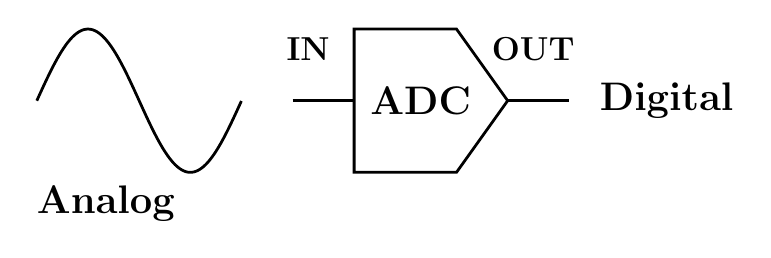
\begin{tikzpicture}[thick, scale=1.3]
        % 類比波形
        \draw[black, line width=1pt, domain=0:2, samples=100] plot (\x, {0.7*sin(180*\x)});
        % Analog 標籤
        \node[anchor=west, text=black, font=\bfseries\Large] at (-0.1,-1) {Analog};
        % 輸入線
        \draw[black, line width=1pt] (2.5,0) -- (3.1,0);
        % ADC 方塊
        \draw[black, line width=1pt] (3.1,0.7) -- (4.1,0.7) -- (4.6,0) -- (4.1,-0.7) -- (3.1,-0.7) -- cycle;
        % IN/OUT 標籤
        \node[text=black, font=\bfseries\large] at (2.65,0.5) {IN};
        \node[text=black, font=\bfseries\large] at (4.85,0.5) {OUT};
        % ADC 字樣
        \node[font=\bfseries\Large, text=black] at (3.75,0) {ADC};
        % 輸出線
        \draw[black, line width=1pt] (4.6,0) -- (5.2,0);
        % Digital 標籤
        \node[anchor=west, text=black, font=\bfseries\Large] at (5.4,0) {Digital};
    \end{tikzpicture}
\end{center}

\vspace{1cm}

% 第二張圖:DAC
\begin{center}
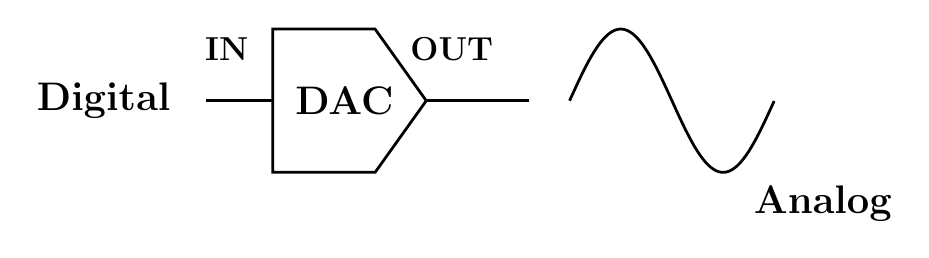
\begin{tikzpicture}[thick, scale=1.3]
    % Digital 標籤
    \node[anchor=east, text=black, font=\bfseries\Large] at (2.2,0) {Digital};
    % 輸入線
    \draw[black, line width=1pt] (2.45,0) -- (3.1,0);
    % DAC 方塊
    \draw[black, line width=1pt] (3.1,0.7) -- (4.1,0.7) -- (4.6,0) -- (4.1,-0.7) -- (3.1,-0.7) -- cycle;
    % IN/OUT 標籤
    \node[text=black, font=\bfseries\large] at (2.65,0.5) {IN};
    \node[text=black, font=\bfseries\large] at (4.85,0.5) {OUT};
    % DAC 字樣
    \node[font=\bfseries\Large, text=black] at (3.8,0) {DAC};
    % 輸出線
    \draw[black, line width=1pt] (4.6,0) -- (5.6,0);
    % 類比波形
    \draw[black, line width=1pt, domain=6:8, samples=100] plot (\x, {0.7*sin(180*(\x-6))});
    % Analog 標籤
    \node[anchor=west, text=black, font=\bfseries\Large] at (7.7,-1) {Analog};
\end{tikzpicture}
\end{center}

\end{document}